\section{Implementación del sistema Odoo}

\subsection{Configuración inicial}

La implementación de la plataforma para Machu Picchu Exclusive Tours se realiza bajo la modalidad Odoo Online (SaaS), lo que permite desplegar una solución centralizada en la nube accesible desde cualquier ubicación. En esta etapa se procedió a la creación del entorno de trabajo, definiendo la base de datos principal, la configuración de moneda (USD y PEN), idioma y zona horaria. Se activaron los módulos de CRM, Proyectos y Ventas, asegurando que el entorno esté preparado para la parametrización de los procesos operativos de la agencia.

\begin{figure}[h]
    \centering
    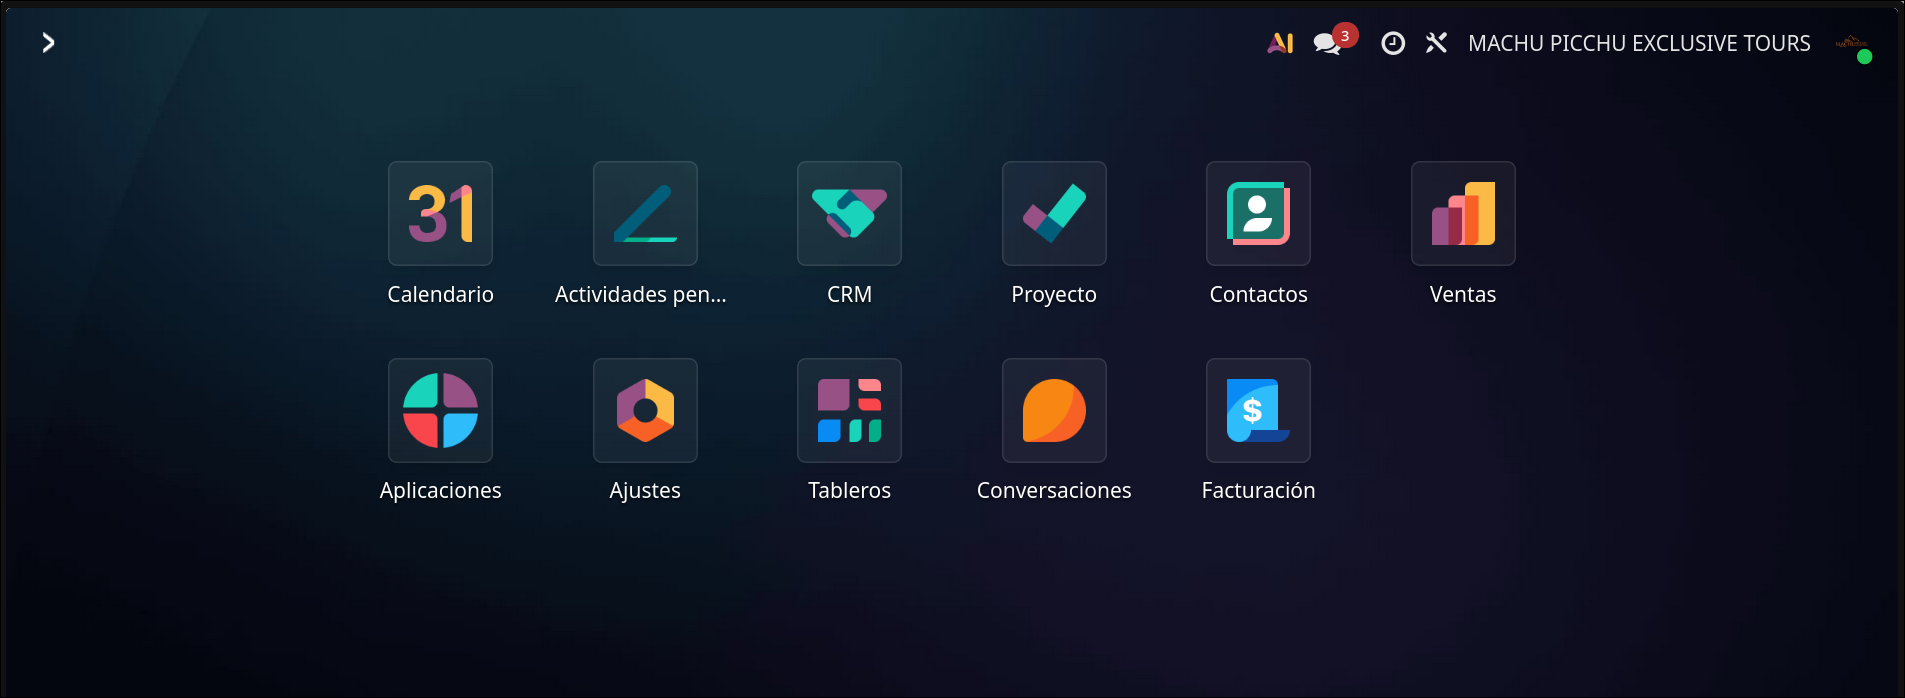
\includegraphics[width=\textwidth]{assets/odoo-configuracion-inicial.png}
    \caption{Configuración inicial de la instancia Odoo Online}
\end{figure}

\subsection{Implementación del módulo CRM (gestión turística)}

El CRM es el núcleo para la centralización de la base de datos de pasajeros (PAX), reemplazando el uso de Excel y WhatsApp. Las acciones clave incluyen:

\begin{itemize}
    \item[a.] \textbf{Almacenamiento seguro de pasaportes}: se habilitó el repositorio estándar para la carga manual y almacenamiento seguro de fotografías de pasaportes y documentos de identidad directamente en la ficha del cliente. Esto elimina el riesgo de seguridad de gestionar datos sensibles en dispositivos personales.
    \item[b.] \textbf{Embudo de ventas (pipeline)}: configuración de un embudo con etapas estándar para el seguimiento de oportunidades comerciales, permitiendo una visión 360° del turista extranjero antes de la confirmación del viaje.
    \item[c.] \textbf{Gestión de interacciones}: registro de notas e historial de comunicaciones para profesionalizar el seguimiento post-cotización.
\end{itemize}

\begin{figure}[h]
    \centering
    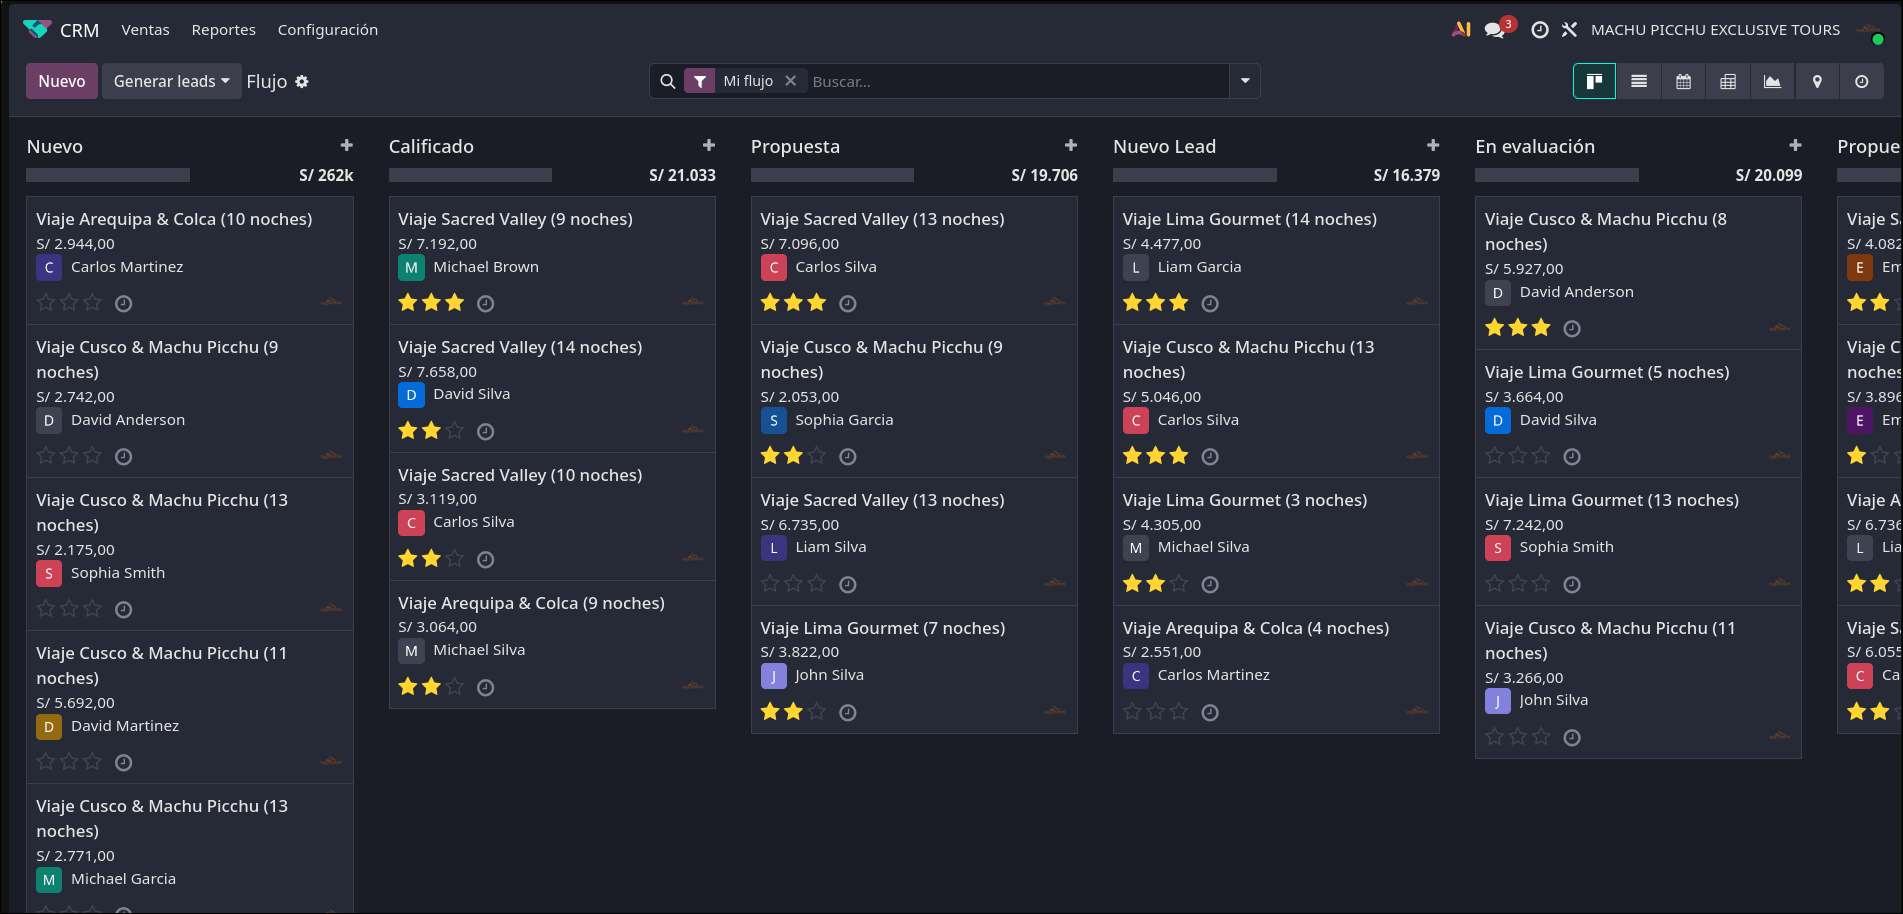
\includegraphics[width=\textwidth]{assets/odoo-crm-pipeline.png}
    \caption{Vista del pipeline de CRM turístico en Odoo}
\end{figure}

\subsection{Implementación del módulo de Proyectos (control de itinerarios)}

Dado que la empresa gestiona itinerarios complejos que varían de 2 a 20 días, se configuró este módulo como herramienta de control operativo:

\begin{itemize}
    \item[a.] \textbf{Tablero visual Kanban}: los servicios se visualizan en un tablero con etapas adaptadas: Borrador de Cotización, Confirmación (Adelanto), Compra de Tickets/Hoteles y Ejecución Final.
    \item[b.] \textbf{Documentación centralizada}: carga manual de boletos de tren, avión y entradas a Machu Picchu como adjuntos en cada tarea, asegurando que toda la evidencia del viaje sea real y accesible.
    \item[c.] \textbf{Asignación de responsables}: permite definir usuarios encargados para el seguimiento de cada reserva, mejorando la coordinación interna.
\end{itemize}

\begin{figure}[h]
    \centering
    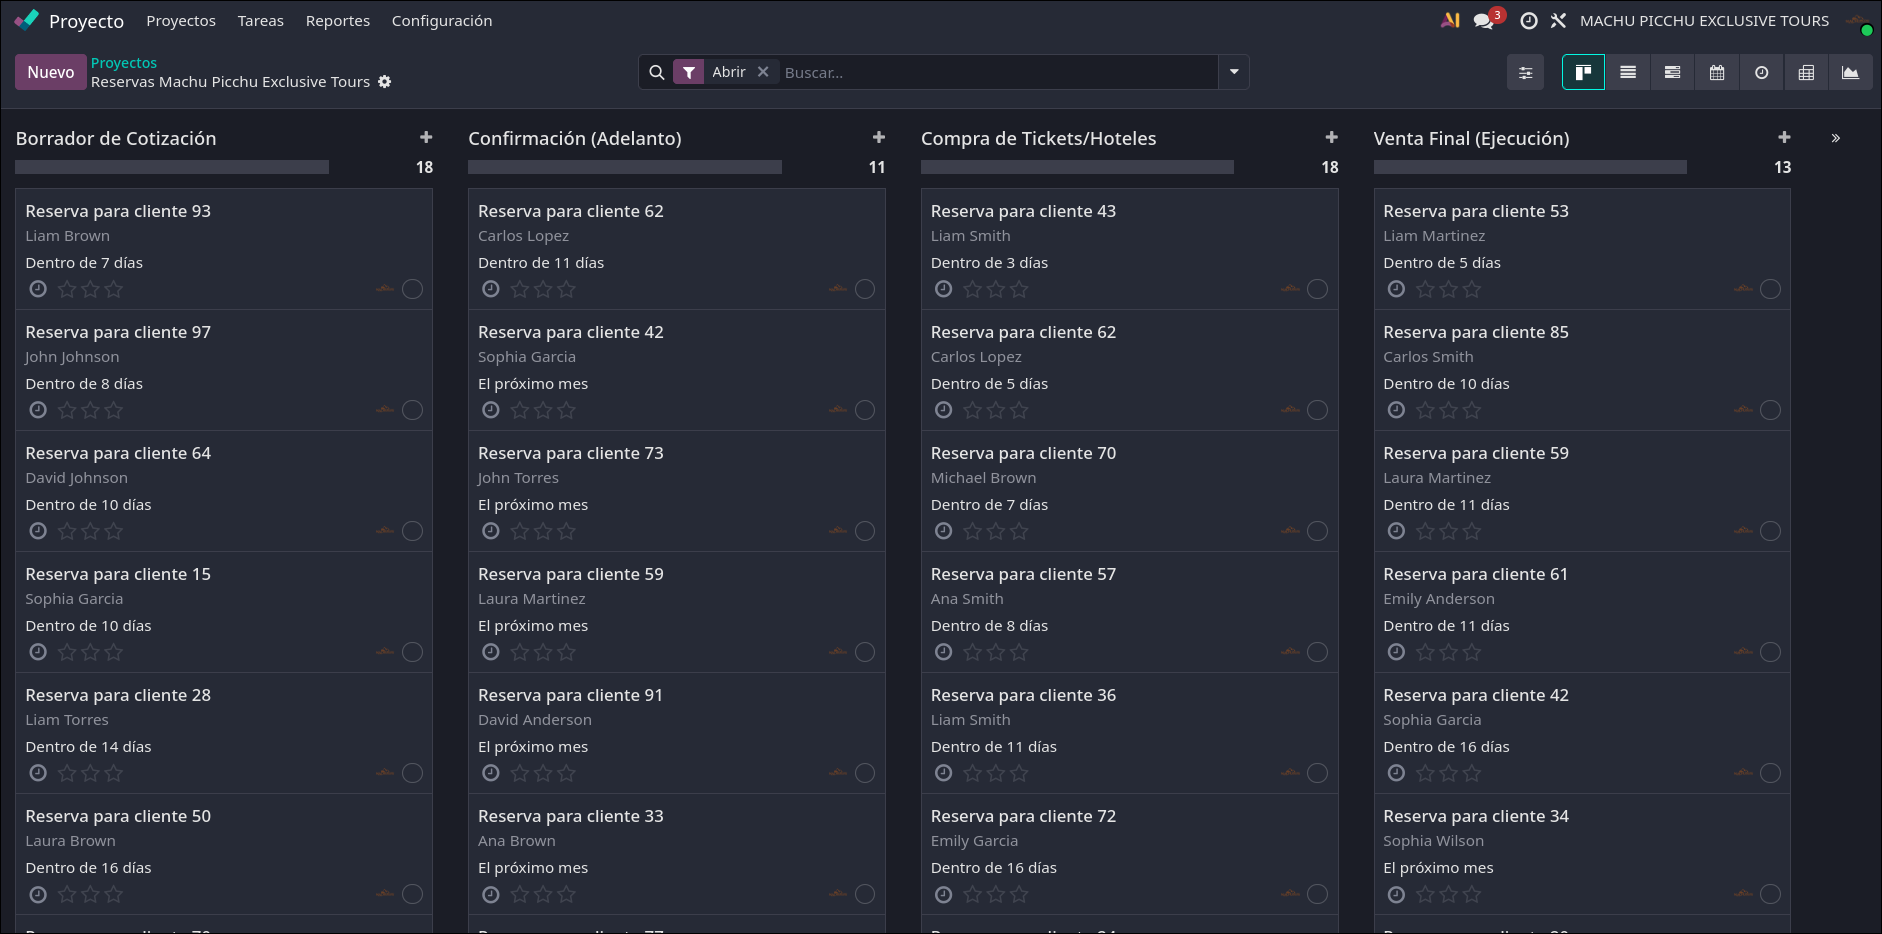
\includegraphics[width=\textwidth]{assets/odoo-proyectos-kanban.png}
    \caption{Tablero Kanban de proyectos para control de itinerarios}
\end{figure}

\subsection{Gestión de cobros y ventas (facturación básica)}

Se parametrizó el flujo de ventas para gestionar los pagos parciales característicos de la agencia:

\begin{itemize}
    \item[a.] \textbf{Registro de adelantos y saldos}: configuración para el registro manual de abonos (usualmente del 30\% al 50\%) cobrados mediante enlaces externos como Ip-App.
    \item[b.] \textbf{Control de saldos pendientes}: el sistema permite visualizar rápidamente si un pasajero tiene saldos por pagar, lo cual es un paso crítico antes de proceder con la compra de boletos no reembolsables.
    \item[c.] \textbf{Confirmaciones automáticas}: generación de recibos internos con el formato estándar de Odoo para enviar la confirmación de recepción de fondos al turista.
\end{itemize}

\begin{figure}[h]
    \centering
    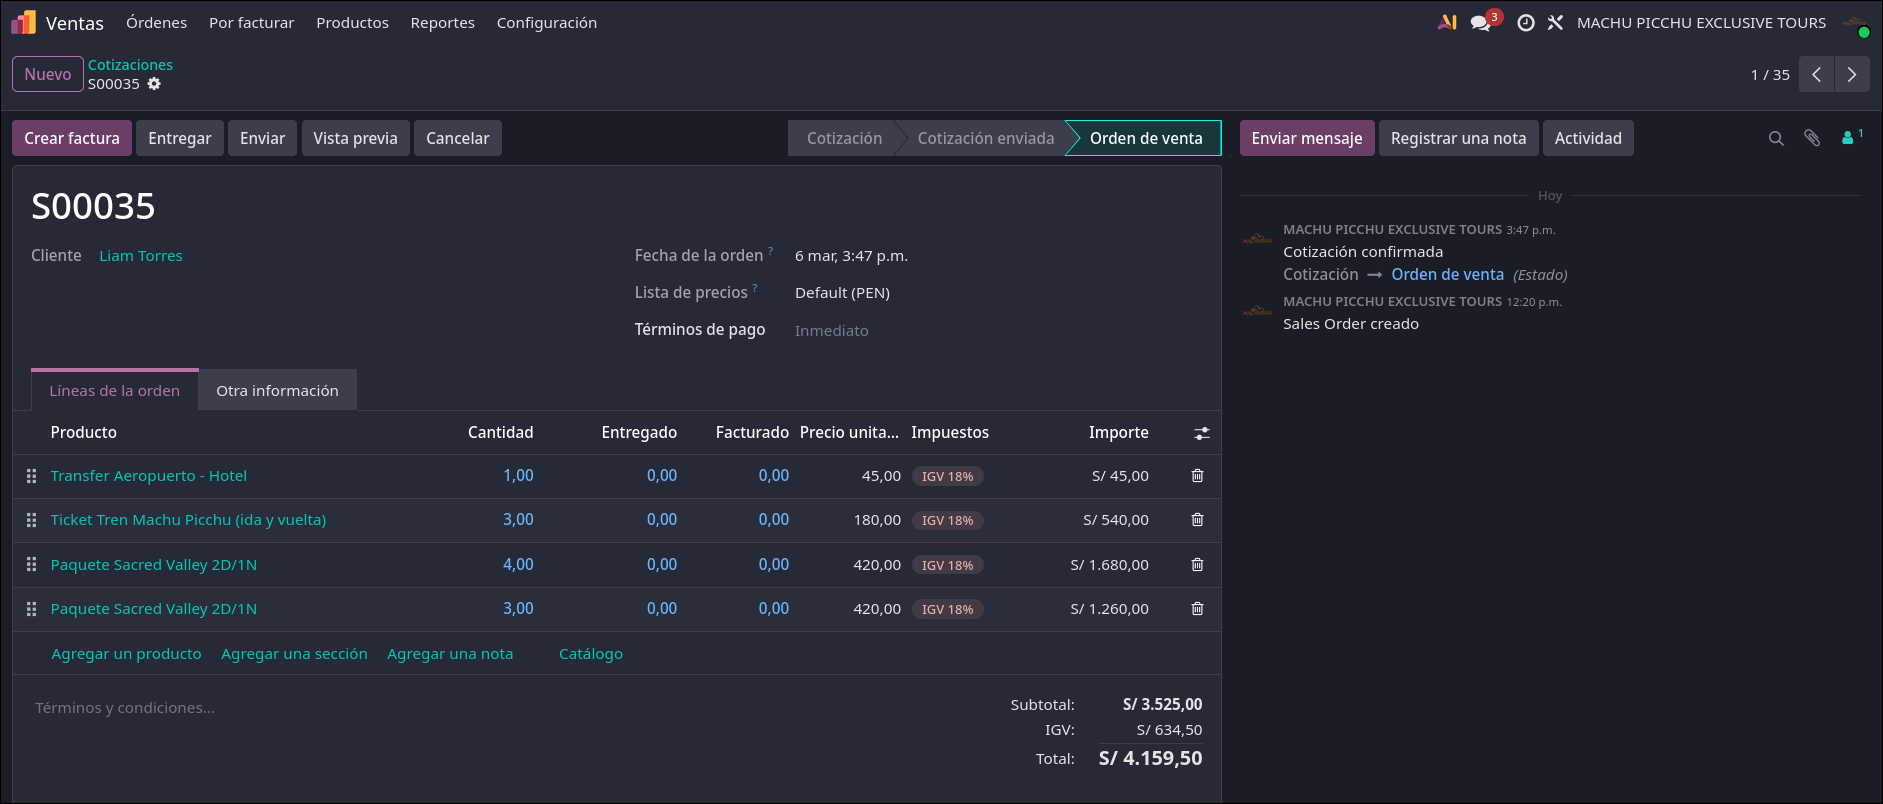
\includegraphics[width=\textwidth]{assets/odoo-facturacion-pagos.png}
    \caption{Gestión de cobros y pagos parciales en Odoo}
\end{figure}

\subsection{Gestión de actividades y alertas}

Se implementó la funcionalidad de \emph{Actividades} para programar recordatorios manuales de llamadas, correos de seguimiento o tareas de post-venta. Estas actividades son visibles en una vista de calendario nativa, facilitando que la gerencia mantenga el contacto personalizado con los clientes (por ejemplo, saludos de cumpleaños o tarjetas de fin de año).

\begin{figure}[h]
    \centering
    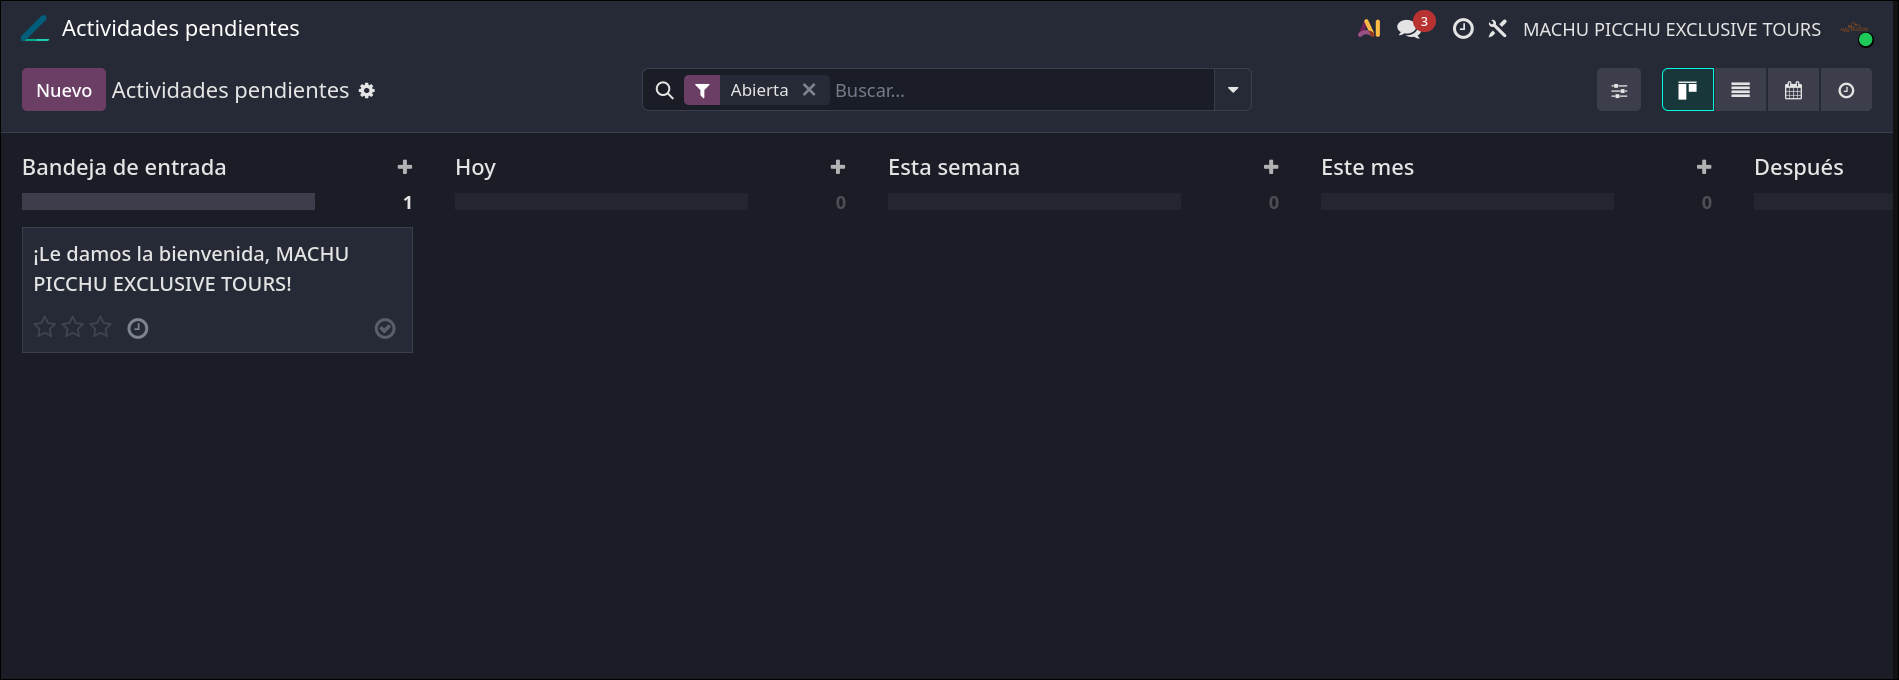
\includegraphics[width=\textwidth]{assets/odoo-actividades.png}
    \caption{Gestión de actividades y recordatorios en Odoo}
\end{figure}

\subsection{Integración entre módulos y trazabilidad del sistema}

La principal fortaleza de esta implementación radica en la interconexión: una oportunidad ganada en el CRM activa automáticamente el seguimiento en el tablero de Proyectos. Esta trazabilidad garantiza que los datos del pasaporte registrados inicialmente se utilicen correctamente en la compra de entradas a Machu Picchu, donde los errores de digitación pueden impedir el ingreso de los turistas debido a las estrictas regulaciones.

\begin{figure}[h]
    \centering
    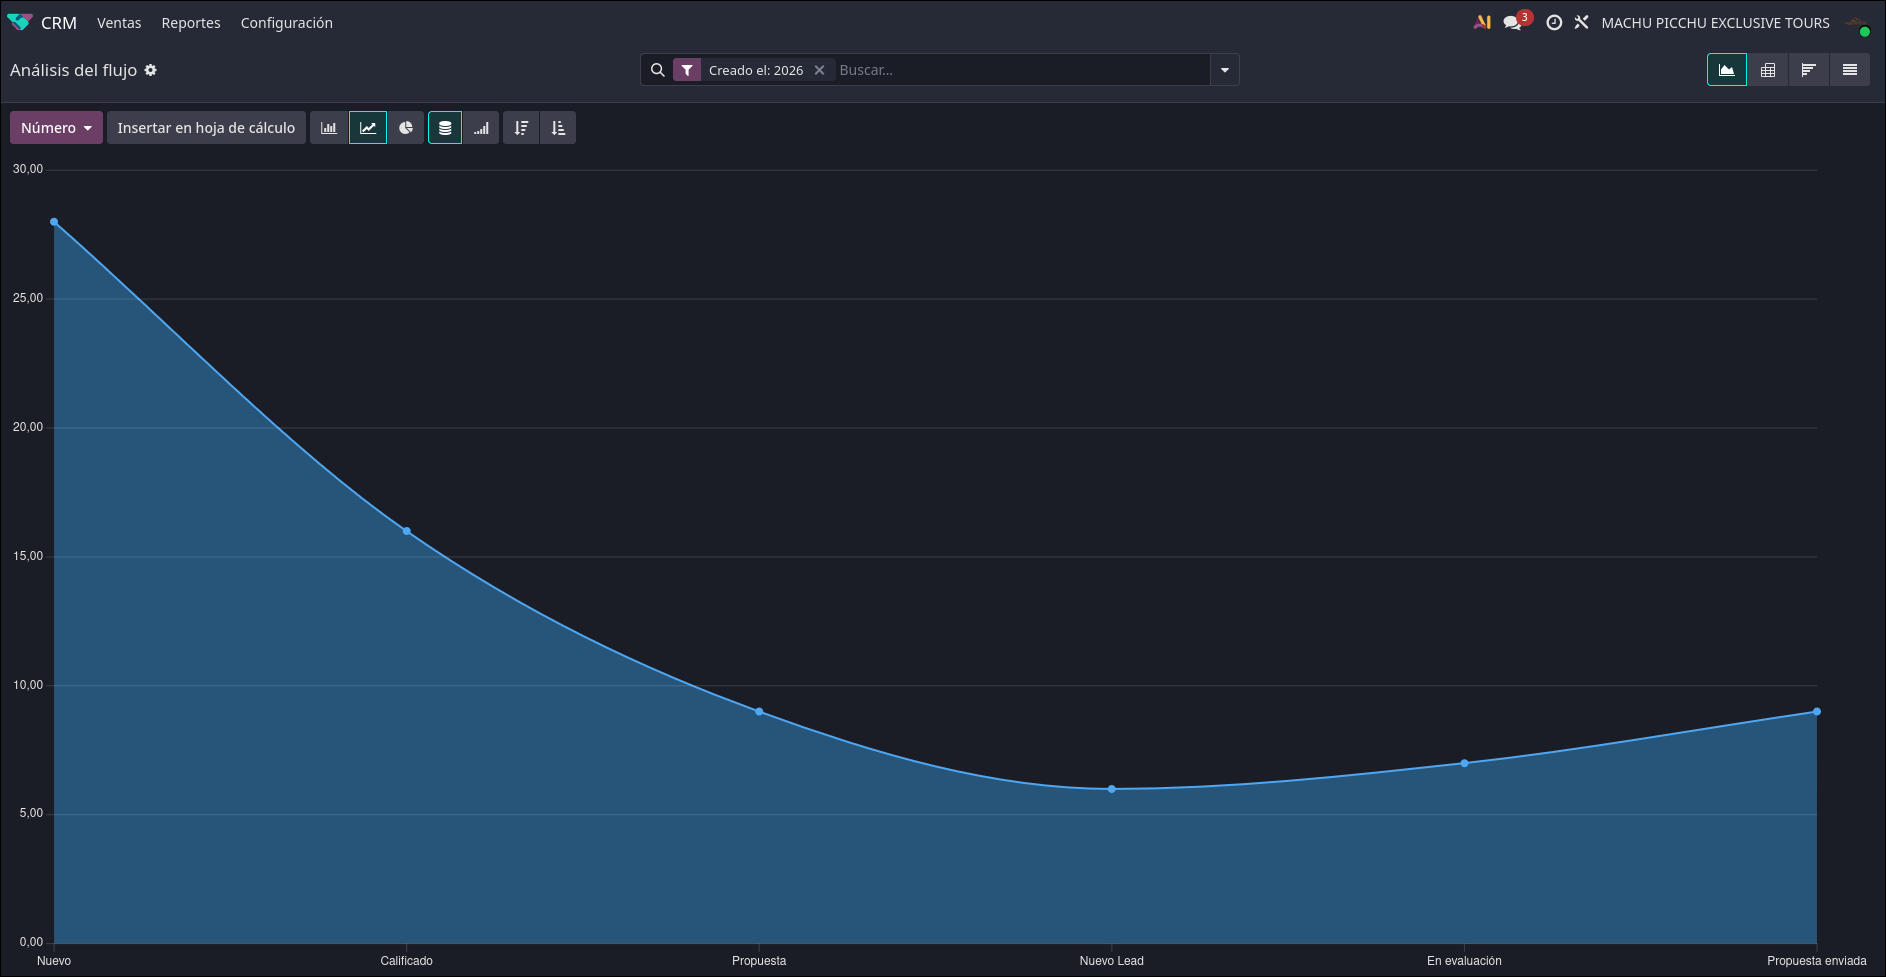
\includegraphics[width=\textwidth]{assets/odoo-trazabilidad-crm-proyectos.png}
    \caption{Trazabilidad entre CRM y Proyectos dentro de Odoo}
\end{figure}

